\chapter{Etwas LaTeX}

In diesem Kapitel sind einige LaTeX-Dinge zusammengesammelt, die immer wieder
auch von Personen verkehrt gemacht werden, die bereits längere Zeit mit LaTeX
arbeiten. Dies soll hier also keine Einführung in LaTeX werden, sondern spiegelt
nur meine Erfahrung der häufigsten Fehler wieder. Außerdem soll gezeigt werden,
wie bestimmte Dinge innerhalb dieser Vorlage gemacht werden.

Grundsätzlich sollte man bei \index{Problem}Problemen nie, nimmer, niemals einfach nach
einer Lösung im Internet suchen. 95\,\% der Lösungen im Internet sind
bestenfalls falsch, aber eigentlich der größte Mist für den die jeweiligen
Autoren angespitzt in den Boden gerammt, im eigen Saft gegart, gevierteilt und
anschließend in Beton gegossen gehören. Aber eigentlich ist es schade um den
guten Beton.

\section{Dokumentationsquellen}

Statt wahllos im Internet nach \index{Losung@Lösung}Lösungen zu suchen, sucht man direkt auf
\url{http://www.ctan.org/tex-archive/} nach dem Paketnamen und verwendet die
dortige Originaldokumentation des Paketautors selbst. Dort zu findende \index{Warnung}Warnungen
sollte man ernst nehmen und nicht machen, auch wenn irgendwo anders behauptet
wird, es würde so funktionieren. Es funktioniert NICHT oder nur scheinbar.

Im Rahmen dieser Vorlage sind insbesondere die \index{Dokumentation}Dokumentationen aus dem
Literaturverzeichnis wärmstens zu empfehlen.

\section{Referenzen}

Querverweise sollten nicht mit dem Befehl \verb#\ref{...}# gesetzt werden sondern
mit \verb#\cref{...}# und verwandten Befehlen aus dem Paket \texttt{cleveref}
\parencite{Cubitt2013}. Diese Befehle haben den Vorteil nicht nur die Nummer
zu referenzieren, sondern auch den Typ mit anzugeben. Hinzukommt eine
intelligente Verwendung der Pluralform und \index{Sortierung}Sortierung bei Mehrfachaufzählungen
auch unterschiedlichen Typs. Will man bspw. auf zwei Abbildungen und eine Tabelle
mit den Marken (\enquote{Labels})
\begin{itemize}
\item \texttt{fig:texniccenter-new-profile-1}
\item \texttt{tab:files-dirs-of-template}
\item \texttt{fig:texniccenter-new-profile-2}
\end{itemize}
verweisen, so schreibt man einfach per Komma getrennt
\begin{latex}[caption={Cleveres Referenzieren},label={lst:cref}]
\cref{fig:texniccenter-new-profile-1,
      tab:files-dirs-of-template,
      fig:texniccenter-new-profile-2}
\end{latex}
und erhält als Resultat \enquote{\cref{fig:texniccenter-new-profile-1,tab:files-dirs-of-template,fig:texniccenter-new-profile-2}}.

\section{Fließumgebungen (Floats)}

Fließumgebungen sind bei LaTeX blockbildende \index{Element!blockbildend}Elemente,
die nicht an der Stelle erscheinen, an der sie im Quellcode definiert sind sondern aus optischen
Gründen an umhergeschoben werden können. Typische Beispiele sind Tabellen,
Bilder, längere Codeausschnitte und ähnliche Dinge. Später wird noch auf
Bilder und Tabellen im Detail eingegangen, aber an diese Stelle sollen vier
Todsünden in Bezug auf Fließumgebungen abgehandelt werden.

Todsünde Nummer eins ist die Verwendung der \index{Platzierung}Platzierungsangabe \texttt{H}, also
bspw.
\begin{latex}[caption={Verbot von \texttt{H} als Platzierungsangabe},label={lst:prohibited-h}]
\begin{figure}[H]
\end{figure}
\end{latex}
um zu erzwingen, dass ein Fließobjekt an dieser Stelle (engl. \enquote{here})
passiert, wenn \texttt{h} nicht genügt. Wenn \texttt{h} nicht genügt, dann liegt
der Fehler bereits woanders und man sollte in das Log schauen, warum LaTeX
die Umgebung nicht platzieren kann und das originäre Problem lösen. Alles andere
macht es nur schlimmer.

Todsünde Nummer zwei ist die Verwendung von Leerzeilen innerhalb der
Fließumgebung oder auch das Abrücken der Fließumgebung mit einer Leerzeile von
dem Text der die Fließumgebung referenziert. Leerzeilen sind bei LaTeX Absätze
und damit potentielle Stellen für Seitenumbrüche. Korrekt ist also folgendes:
\begin{latex}[caption={Verbot von Leerzeilen},label={lst:prohibited-blank-lines}]
Ein Text der auf die \cref{fig:my-fig} verweist
\begin{figure}[htbp]
  \centering
  \includegraphics{./images/my-image.png}
  \caption{Eine tolle Abbildung}
  \label{fig:my-fig}
\end{figure}
und ohne Leerzeile an der figure-Umgebung dransteht.

Dies ist nun ein neuer Absatz.
\end{latex}
Wie man erkennen kann, steht die \texttt{figure}-Umgebung sogar mitten im Satz
zu der sie gehört. Der häufigste Grund, warum die Platzierungsoptionen
\texttt{t}, \texttt{b}, \texttt{h} und  \texttt{p} nicht so verhalten, wie
man erwartet, ist, dass die \texttt{figure}-Umgebung aus Gründen der Übersicht
mit Leerzeilen abgesetzt wird, sodass diese dann für LaTeX einen eigenen Block
bildet.

Todsünde Nummer drei ist die Verwendung von \verb#\begin{center}# und
\verb#\end{center}# statt von \verb#\centering# innerhalb der Fließumgebung.
Ersteres erzeugt wieder einen internen Absatz und damit einen eigenen Block.
Dies ist also genauso schlimm wie Leerzeilen.

Todsünde Nummer vier ist die falsche Reihenfolge von \verb#\caption{...}# und
\verb#\label{...}#. Die Reihenfolge ist \emph{immer} das Objekt selbst (also
\verb#\includegraphics# oder \verb#tabular#, usw.), dann folgt \verb#\caption{...}#
und zum Schluss \verb#\label{...}#.

\section{Tabellen}

Typografisch gute Tabellen haben \emph{niemals} vertikale Trennlinien sondern
nur wenige horizontale Linien. Ferner haben sie eine trennende Linie ganz oben
und ganz unten. Hierfür stellt das Paket \texttt{booktabs} die Befehle
\begin{itemize}
  \item \verb#\toprule#
	\item \verb#\midrule#
	\item \verb#\bottomrule#
\end{itemize}
zur Verfügung. Der Befehl \verb#\hline# ist tabu. Für eine ausführliche
Erläuterung auch über gute und schlechte Tabellen siehe die Dokumentation des
\texttt{booktabs}-Pakets \parencite{Fear2005}.

Eine gute Tabelle hat also folgenden Code
\begin{latex}[caption={Tabellen in LaTeX},label={lst:tables}]
\begin{table}
  \centering
  \begin{tabular}{l l l}                       \toprule
    Datei       &  Bedeutung    &  Benutzer \\ \midrule
    ./main.tex  &  Hauptdatei   &  nein     \\
    ./figures/  &  Zeichnungen  &  ja       \\
    ./content/  &  Kapitel      &  ja       \\
    ./logos/    &  Logos        &  nein     \\ \bottomrule
  \end{tabular}
  \caption{Dateien der Vorlage}
  \label{tab:files-dirs-of-template}
\end{table}
\end{latex}
und sieht dann so aus wie \cref{tab:files-dirs-of-template}.

Sollten eine Tabelle einmal so breit sein, dass sie nicht mehr horizontal auf
eine Seite passt, so ist es natürlich möglich, diese mithilfe des Pakets
\texttt{rotfloat} \parencite{Sommerfeldt2004} statt in eine \texttt{table}- in eine
\texttt{sidewaystable}-Umgebung zu setzen. Also
\begin{latex}[caption={Gedrehte Tabelle},label={lst:rotated-table}]
\begin{sidewaystable}
  \centering
  \begin{tabular}{...}
    ...
  \end{tabular}
  \caption{Bezeichnung}
  \label{Referenzmarke}
\end{sidewaystable}
\end{latex}
ein Ergebnis sieht man in \cref{tab:ex-sideways}.
\newcolumntype{M}{>{\begin{minipage}[t]{2.7cm}\raggedright}c<{\end{minipage}}}
\newenvironment{tabitemize}{%
\begin{list}{\textbullet}{%
\setlength\topsep{0pt}%
\setlength\parsep{0pt}%
\setlength\itemsep{0pt}%
\setlength\leftmargin{0em}%
\setlength\leftmargin{1em}%
\setlength\labelwidth{0.5em}%
\setlength\labelsep{0.5em}%
}
}{%
\end{list}
}
\begin{sidewaystable}[p]
\scriptsize
\centering
\begin{tabular}{l M M M M M} \toprule\addlinespace[0pt]
 & \multicolumn{5}{c}{\bfseries Level} \tabularnewline
 & \multicolumn{2}{c}{\bfseries Qualitative} & \multicolumn{3}{c}{\bfseries Quantitative} \tabularnewline
 & \bfseries\centering Nominal & \bfseries\centering Ordinal & \bfseries\centering Interval & \bfseries\centering Ratio & \bfseries\centering Absolute \tabularnewline \addlinespace[0pt]\midrule\addlinespace[0pt]
Empirical relation &
\begin{tabitemize}\item[$\sim$] Equivalence\end{tabitemize} &
\begin{tabitemize}\item[$\sim$] Equivalence\item[$\prec$] Ordering\end{tabitemize} &
\begin{tabitemize}\item[$\sim$] Equivalence\item[$\prec$] Ordering\end{tabitemize} &
\begin{tabitemize}\item[$\sim$] Equivalence\item[$\prec$] Ordering\strut\end{tabitemize} &
\begin{tabitemize}\item[$\sim$] Equivalence\item[$\prec$] Ordering\strut\end{tabitemize} \tabularnewline \midrule
Empirical operation &
 &
 &
\begin{tabitemize}\item[$\oplus$] Addition\end{tabitemize} &
\begin{tabitemize}\item[$\oplus$] Addition\item[$\otimes$] Multiplication\strut\end{tabitemize} &
\begin{tabitemize}\item[$\oplus$] Addition\item[$\otimes$] Multiplication\strut\end{tabitemize} \tabularnewline \midrule
Feasable transformation &
$m' = f( m )$ for $f$ bij.\strut &
$m' = f( m )$ for $f$ mon.\strut &
$m' = am + b$ for $a>0$\strut &
$m' = am$ for $a>0$\strut &
$m' = m$\strut \tabularnewline \midrule
Examples of features &
\begin{tabitemize}\item Telephone numbers\item Postal codes\item Gender\strut\end{tabitemize} &
\begin{tabitemize}\item Grades\item Degree of hardness\item Wind intensity\strut\end{tabitemize} &
\begin{tabitemize}\item Temperatur in F\textdegree\item Calendric time\item Geographic altitude\strut\end{tabitemize} &
\begin{tabitemize}\item Temperatur in K\item Mass\item Length\item Electric current\strut\end{tabitemize} &
\begin{tabitemize}\item Quantum numbers\item Error number\strut\end{tabitemize} \tabularnewline \midrule
Range of features &
\begin{tabitemize}\item Numbers\item Names\item Symbols\strut\end{tabitemize} &
Natural numbers &
Real numbers &
Real, positive numbers &
Natural numbers \tabularnewline \midrule
Expressiveness & low & \dots & \dots & \dots & high\strut \tabularnewline \addlinespace[0pt]\bottomrule
\end{tabular}
\caption{Beispiel für eine breite, gedrehte Tabelle (hier: Taxonomie der Maßskalen)}
\label{tab:ex-sideways}
\end{sidewaystable}

\section{Bilder, Grafiken und Diagramme}

Bei Grafiken sind zwei Fälle zu unterscheiden:
\begin{itemize}
  \item \index{Bild!Binär-}Bilder in einem Binärformat (\texttt{PNG}, \texttt{TIFF}, \texttt{JPG}, \texttt{PDF}, etc.)
	\item \index{Bild!Vektor-}Grafiken, die im \gls{tikz}-Quellcode vorliegen 
\end{itemize}
Grundlegender Unterschied ist, dass Binärformatgrafiken mit \verb#\includegraphics#
eingebunden werden während \gls{tikz}-Grafiken mit \verb#\input# eingebunden und
von \texttt{pdflatex} kompiliert werden.

Für Binärformatbilder ist ein vollständiges Beispiel also
\begin{latex}[caption={Binärgrafik in LaTeX},label={lst:binary-image}]
\begin{figure}[htbp]
  \centering
  \includegraphics{./images/my-image.png}
  \caption{Eine tolle Abbildung}
  \label{fig:my-image}
\end{figure}
\end{latex}
Der Code für eine \gls{tikz}-Grafik ist hingegen
\begin{latex}[caption={TikZ-Zeichnung in LaTeX},label={lst:tikz-figure}]
\begin{figure}[htbp]
  \centering
	\tikzsetnextfilename{my-tikz-figure}
  \input{./figures-src/my-tikz-figure.tex}
  \caption{Eine tolle Zeichnung}
  \label{fig:my-figure}
\end{figure}
\end{latex}
Das Kommando \verb#\tikzsetnextfilename{...}# ist nicht unbedingt notwendig
aber sehr zu empfehlen, da dies als Name für das temporäre Kompilat im Ordner
\texttt{./figures-compiled/} genommen wird. Dieser sollte gleich dem Namen
des Quelldatei (ohne Endung) gewählt werden. Ansonsten nimmt \texttt{pdflatex}
eine hochlaufende Nummer als Dateiname, was die Fehlersuche sehr erschwert.

Bilder können auch in
\index{Abbildung|see{Bild}}\index{Bild!Unterabbildung}Unterabbildungen gesetzt
und sowohl als ganzes
\begin{figure}[tbp]\centering
\subfloat[La Savoureuse, Lepuix, Frankreich (\copyright\ Thomas Bresson)]{
  \label{fig:subfloat-example-01}
	\includegraphics{./images/subfloat-example-01.jpg}
} \qquad
\subfloat[Bangkok, Thailand (\copyright\ Prachanart Viriyaraks)]{
  \label{fig:subfloat-example-02}
	\includegraphics{./images/subfloat-example-02.jpg}
} \\
\subfloat[Wahkeena Falls, Lincoln Park, USA (\copyright\ srslyguys)]{
  \label{fig:subfloat-example-03}
	\includegraphics{./images/subfloat-example-03.jpg}
} \qquad
\subfloat[Nacionalni park Plitvička jezer, Kroatien (\copyright\ Roman Bonnefoy)]{
  \label{fig:subfloat-example-04}
	\includegraphics{./images/subfloat-example-04.jpg}
}
\caption{Wasserfälle der Welt als Beispiel für Unterabbildungen}
\label{fig:subfloat-example}
\end{figure}
(vgl. \cref{fig:subfloat-example}) als auch einzeln (vgl.
\cref{fig:subfloat-example-01,fig:subfloat-example-02,fig:subfloat-example-03,fig:subfloat-example-04})
referenziert werden. Der Beispielcode mit dem Paket \texttt{Subfig}
\parencite{Cochran2005} hierzu ist
\begin{latex}[caption={Unterabbildungen in LaTeX},label={lst:subfigures}]
\begin{figure}
\centering
\subfloat[Unterbezeichnung 1)]{
  \label{fig:my-sub-figure-1}
	\includegraphics{./Pfad/zu/Bild/1}
} \qquad
\subfloat[Unterbezeichnung 2]{
  \label{fig:my-sub-figure-2}
	\includegraphics{./Pfad/zu/Bild/2}
}
\caption{Bezeichnung}
\label{fig:my-whole-figure}
\end{figure}
\end{latex}

\Gls{tikz} eignet sich hervorragend, um wissenschaftliche Zeichnungen, Vektorgrafiken
und \index{Diagramm}Diagramme direkt mithilfe von LaTeX zu setzen, sodass die Schrift direkt zum
restlichen Dokument passt. Zu \gls{tikz} und dem darauf aufsetzenden \gls{pgfplots} gibt
es hervorragende Dokumentation \parencites{Tantau2013}{Feuersaenger2014}.


Möglich sind zum Beispiel einfache \index{Diagramm!Punkt-}Punktdiagramme wie in \cref{fig:ica} oder
aufwendigere Diagramme mit mehreren \index{Achsensystem|see{Diagramm}}Achsensystemen wie in \cref{fig:pca}.
\begin{figure}[tbp]\centering
\subfloat[Ursprünglicher Merkmalsraum]{
  \label{fig:ica-1}
	\tikzsetnextfilename{ica-1}
	\begin{tikzpicture}[
my_plot/.style={draw=none,every mark/.append style={draw=KITblue,fill=KITblue},mark=*,mark size=1.5pt},
]

\begin{axis}[
width=4cm,
height=4cm,
xmin = -1.1,
xmax = 1.1,
xlabel={$m_1$},
ymin = -1.1,
ymax = 1.1,
ylabel={$m_2$},
axis lines=center,
scale only axis,
]

\addplot[my_plot] coordinates {
(0.030,-0.062) (-0.118,-0.004) (0.276,0.236) (0.578,0.566) (-0.143,-0.014)
(0.304,0.257) (0.423,0.535) (0.205,0.344) (0.364,0.365) (-0.327,-0.368)
(0.176,0.310) (-0.298,-0.360) (0.153,0.279) (0.010,0.062) (0.150,0.231)
(-0.301,-0.214) (0.079,0.094) (-0.241,-0.161) (-0.474,-0.461) (0.091,0.173)
(0.541,0.601) (-0.288,-0.153) (0.013,-0.093) (0.290,0.115) (0.194,0.028)
(0.486,0.370) (0.201,0.227) (0.510,0.510) (-0.211,-0.293) (-0.058,0.088)
(0.326,0.176) (-0.591,-0.574) (0.071,0.204) (-0.401,-0.308) (0.206,0.111)
(-0.529,-0.667) (0.064,0.040) (0.032,0.035) (-0.349,-0.291) (0.476,0.316)
(0.625,0.624) (0.312,0.234) (0.076,-0.079) (0.016,0.018) (-0.556,-0.655)
(-0.308,-0.217) (0.248,0.122) (-0.515,-0.428) (-0.121,0.041) (0.260,0.228)
(-0.317,-0.406) (0.650,0.483) (-0.198,-0.097) (-0.427,-0.495) (0.429,0.553)
(-0.432,-0.538) (-0.460,-0.440) (-0.558,-0.654) (0.516,0.586) (-0.230,-0.205)
(0.148,0.199) (-0.417,-0.240) (-0.138,-0.040) (-0.252,-0.403) (0.096,0.010)
(-0.478,-0.339) (0.628,0.650) (0.054,-0.104) (0.502,0.429) (0.051,0.045)
(0.099,0.106) (0.344,0.214) (-0.359,-0.334) (0.291,0.187) (0.176,0.217)
(0.329,0.362) (-0.270,-0.116) (-0.136,-0.008) (-0.446,-0.533) (0.653,0.585)
(0.474,0.540) (0.093,0.136) (0.356,0.473) (0.232,0.217) (0.592,0.659)
(-0.326,-0.170) (-0.683,-0.497) (-0.484,-0.357) (-0.607,-0.635) (-0.044,-0.041)
(-0.681,-0.533) (-0.306,-0.401) (0.189,0.334) (0.420,0.259) (0.040,0.086)
(-0.148,-0.303) (-0.585,-0.507) (0.424,0.330) (0.597,0.688) (0.211,0.271)
(-0.429,-0.360) (0.280,0.188) (0.375,0.252) (-0.505,-0.528) (-0.064,-0.043)
(-0.257,-0.140) (0.302,0.262) (-0.228,-0.293) (0.154,0.122) (-0.549,-0.403)
(0.034,-0.027) (0.207,0.122) (-0.538,-0.648) (-0.601,-0.664) (-0.623,-0.433)
(-0.552,-0.417) (-0.094,-0.166) (0.469,0.496) (0.580,0.497) (0.212,0.159)
(0.515,0.627) (-0.070,-0.167) (-0.101,-0.015) (-0.244,-0.328) (-0.372,-0.477)
(0.256,0.199) (-0.607,-0.560) (-0.462,-0.554) (0.132,0.086) (0.066,0.050)
(0.230,0.157) (-0.502,-0.556) (0.666,0.490) (0.407,0.425) (-0.219,-0.355)
(-0.250,-0.285) (0.266,0.159) (-0.263,-0.412) (0.028,0.091) (-0.086,0.043)
(-0.633,-0.504) (-0.420,-0.399) (0.378,0.380) (-0.008,-0.163) (-0.226,-0.278)
(0.148,0.193) (-0.629,-0.582) (0.586,0.450) (0.025,0.136) (-0.445,-0.360)
};

\end{axis}
\end{tikzpicture}
} \quad
\subfloat[Transienter Merkmalsraum (Nach Whitening, z.\,B. durch \glstext{pca} inkl. Normalisierung)]{
  \label{fig:ica-2}
	\tikzsetnextfilename{ica-2}
	\begin{tikzpicture}[
my_plot/.style={draw=none,every mark/.append style={draw=KITblue,fill=KITblue},mark=*,mark size=1.5pt},
]

\begin{axis}[
width=4cm,
height=4cm,
xmin = -1.1,
xmax = 1.1,
xlabel={$m'_1$},
ymin = -1.1,
ymax = 1.1,
ylabel={$m'_2$},
axis lines=center,
scale only axis,
]

\addplot[my_plot] coordinates {
(-0.273,-0.278) (0.267,0.398) (0.117,-0.289) (0.483,-0.399) (0.293,0.455)
(0.120,-0.326) (0.747,0.049) (0.640,0.265) (0.329,-0.231) (-0.430,0.090)
(0.597,0.269) (-0.471,0.014) (0.549,0.259) (0.180,0.141) (0.401,0.136)
(0.014,0.439) (0.120,-0.008) (0.044,0.379) (-0.384,0.338) (0.349,0.173)
(0.681,-0.175) (0.183,0.566) (-0.335,-0.309) (-0.310,-0.678) (-0.368,-0.593)
(0.057,-0.637) (0.266,-0.054) (0.457,-0.325) (-0.457,-0.098) (0.425,0.450)
(-0.196,-0.631) (-0.474,0.426) (0.500,0.334) (-0.059,0.516) (-0.127,-0.402)
(-0.926,-0.054) (-0.019,-0.107) (0.038,-0.012) (-0.122,0.388) (-0.094,-0.754)
(0.560,-0.398) (0.026,-0.418) (-0.439,-0.488) (0.021,-0.004) (-0.822,0.075)
(0.020,0.454) (-0.190,-0.516) (-0.180,0.573) (0.420,0.535) (0.130,-0.255)
(-0.575,-0.050) (0.039,-0.885) (0.151,0.410) (-0.607,0.078) (0.790,0.077)
(-0.736,-0.026) (-0.348,0.349) (-0.817,0.082) (0.692,-0.130) (-0.126,0.216)
(0.301,0.052) (0.202,0.765) (0.195,0.363) (-0.719,-0.267) (-0.195,-0.306)
(0.024,0.696) (0.635,-0.338) (-0.469,-0.483) (0.215,-0.523) (0.028,-0.048)
(0.113,-0.042) (-0.116,-0.587) (-0.242,0.298) (-0.078,-0.479) (0.291,0.003)
(0.405,-0.114) (0.259,0.605) (0.297,0.450) (-0.684,0.038) (0.365,-0.607)
(0.644,-0.112) (0.223,0.062) (0.701,0.104) (0.158,-0.192) (0.752,-0.185)
(0.214,0.646) (-0.007,0.960) (-0.020,0.667) (-0.635,0.308) (-0.029,0.037)
(-0.131,0.849) (-0.587,-0.076) (0.645,0.292) (-0.150,-0.724) (0.184,0.102)
(-0.638,-0.344) (-0.270,0.594) (0.073,-0.536) (0.833,-0.122) (0.385,0.036)
(-0.160,0.468) (-0.048,-0.437) (-0.065,-0.586) (-0.531,0.254) (0.010,0.099)
(0.151,0.495) (0.141,-0.305) (-0.417,-0.039) (0.033,-0.188) (-0.016,0.763)
(-0.166,-0.191) (-0.093,-0.373) (-0.843,0.031) (-0.746,0.204) (0.060,0.933)
(-0.055,0.733) (-0.320,-0.144) (0.510,-0.221) (0.252,-0.601) (0.018,-0.283)
(0.829,-0.011) (-0.381,-0.230) (0.190,0.308) (-0.492,-0.081) (-0.679,-0.062)
(0.042,-0.326) (-0.391,0.520) (-0.717,0.032) (-0.032,-0.214) (0.009,-0.085)
(-0.034,-0.355) (-0.627,0.168) (0.022,-0.923) (0.424,-0.209) (-0.641,-0.245)
(-0.339,0.060) (-0.110,-0.472) (-0.722,-0.253) (0.230,0.160) (0.345,0.421)
(-0.147,0.768) (-0.309,0.326) (0.348,-0.233) (-0.513,-0.434) (-0.372,-0.002)
(0.278,0.031) (-0.413,0.531) (0.082,-0.757) (0.384,0.297) (-0.122,0.523)
};

\end{axis}
\end{tikzpicture}
} \quad
\subfloat[Transformierter Merkmalsraum]{
  \label{fig:ica-3}
	\tikzsetnextfilename{ica-3}
	\begin{tikzpicture}[
my_plot/.style={draw=none,every mark/.append style={draw=KITblue,fill=KITblue},mark=*,mark size=1.5pt},
]

\begin{axis}[
width=4cm,
height=4cm,
xmin = -1.1,
xmax = 1.1,
xlabel={$m''_1$},
ymin = -1.1,
ymax = 1.1,
ylabel={$m''_2$},
axis lines=center,
scale only axis,
]

\addplot[my_plot] coordinates {
(-0.389,-0.004) (0.470,0.093) (-0.122,-0.287) (0.059,-0.623) (0.529,0.115)
(-0.146,-0.316) (0.563,-0.493) (0.640,-0.265) (0.069,-0.396) (-0.241,0.367)
(0.613,-0.232) (-0.323,0.342) (0.572,-0.205) (0.227,-0.027) (0.379,-0.188)
(0.320,0.300) (0.079,-0.090) (0.299,0.237) (-0.033,0.510) (0.369,-0.124)
(0.358,-0.605) (0.530,0.271) (-0.455,0.019) (-0.699,-0.260) (-0.680,-0.159)
(-0.410,-0.491) (0.150,-0.226) (0.093,-0.554) (-0.393,0.254) (0.619,0.017)
(-0.584,-0.307) (-0.034,0.636) (0.590,-0.118) (0.323,0.406) (-0.374,-0.194)
(-0.693,0.617) (-0.089,-0.062) (0.018,-0.035) (0.188,0.361) (-0.600,-0.467)
(0.114,-0.678) (-0.277,-0.314) (-0.655,-0.035) (0.012,-0.018) (-0.528,0.634)
(0.335,0.306) (-0.499,-0.230) (0.278,0.532) (0.676,0.081) (-0.088,-0.272)
(-0.442,0.371) (-0.599,-0.654) (0.397,0.183) (-0.374,0.484) (0.613,-0.504)
(-0.539,0.502) (0.001,0.493) (-0.520,0.635) (0.398,-0.581) (0.063,0.242)
(0.249,-0.176) (0.684,0.398) (0.395,0.119) (-0.697,0.320) (-0.354,-0.078)
(0.509,0.475) (0.210,-0.688) (-0.674,-0.010) (-0.218,-0.522) (-0.014,-0.053)
(0.050,-0.110) (-0.498,-0.333) (0.040,0.382) (-0.394,-0.284) (0.208,-0.204)
(0.206,-0.367) (0.611,0.245) (0.528,0.108) (-0.457,0.510) (-0.171,-0.688)
(0.376,-0.535) (0.202,-0.114) (0.569,-0.422) (-0.024,-0.247) (0.401,-0.663)
(0.608,0.305) (0.674,0.684) (0.457,0.486) (-0.231,0.667) (0.005,0.047)
(0.508,0.693) (-0.469,0.362) (0.663,-0.250) (-0.618,-0.406) (0.203,-0.058)
(-0.694,0.208) (0.229,0.611) (-0.327,-0.431) (0.503,-0.676) (0.298,-0.247)
(0.217,0.444) (-0.343,-0.275) (-0.460,-0.368) (-0.196,0.555) (0.077,0.063)
(0.457,0.243) (-0.116,-0.315) (-0.322,0.267) (-0.110,-0.157) (0.528,0.550)
(-0.253,-0.018) (-0.329,-0.198) (-0.574,0.618) (-0.384,0.672) (0.702,0.617)
(0.480,0.557) (-0.329,0.124) (0.205,-0.517) (-0.247,-0.604) (-0.188,-0.213)
(0.578,-0.594) (-0.432,0.106) (0.352,0.083) (-0.406,0.291) (-0.523,0.436)
(-0.201,-0.260) (0.091,0.644) (-0.484,0.530) (-0.173,-0.129) (-0.054,-0.067)
(-0.275,-0.227) (-0.325,0.562) (-0.637,-0.668) (0.152,-0.447) (-0.626,0.280)
(-0.197,0.283) (-0.411,-0.256) (-0.690,0.332) (0.276,-0.050) (0.542,0.054)
(0.439,0.647) (0.012,0.449) (0.081,-0.411) (-0.670,0.056) (-0.265,0.262)
(0.218,-0.175) (0.083,0.668) (-0.477,-0.594) (0.482,-0.061) (0.284,0.456)
};

\end{axis}
\end{tikzpicture}
}
\caption{Diagramme mit TikZ direkt in LaTeX (hier: Die Schritte der \enquote{Independent component analysis})}
\label{fig:ica}
\end{figure}
\begin{figure}[tbp]\centering
\subfloat[Ungünstige Projektion]{
  \label{fig:pca-1}
  \tikzsetnextfilename{pca-1}
  \begin{tikzpicture}[
my_plot_1/.style={draw=none,every mark/.append style={draw=KITblue,fill=KITblue},mark=*},
my_plot_2/.style={draw=none,every mark/.append style={draw=KITred,fill=KITred},mark=*},
trans_arrow/.style={semithick,KITorange,-latex},
]

\begin{axis}[
width=4cm,
height=4cm,
xmin = -0.2,
xmax = 2.3,
xlabel={$m_1$},
ymin = -0.2,
ymax = 2.3,
ylabel={$m_2$},
xticklabel=\empty,
yticklabel=\empty,
axis lines=center,
clip=false,
scale only axis,
]

\addplot[my_plot_1] coordinates {
(1.3,0.38)
(1.42,0.71)
(1.48,0.60)
(1.64,0.54)
(1.65,0.81)
(1.68,0.89)
(1.79,1.11)
(1.88,1.18)
(1.89,1.46)
(1.94,1.35)
(1.86,1.65)
(2.02,1.83)
(2.12,1.83)
(2.19,2.26)
(2.21,2.07)
};

\addplot[my_plot_2] coordinates {
(1.28,0.58)
(1.33,0.93)
(1.54,1.03)
(1.54,1.26)
(1.51,1.41)
(1.72,1.52)
(1.76,1.87)
(1.80,1.90)
(1.90,2.00)
(1.91,2.27)
(2.05,2.40)
};

\coordinate(CoM) at (axis cs:1.71,1.38) {};

\draw[trans_arrow] (axis cs:0,0)--(CoM) node[midway,above left] {$m_0$};

\end{axis}

\begin{axis}[
width=5cm,
height=2.5cm,
xmin = -1.5,
xmax = 1.5,
xlabel={$m'_1$},
ymin = -0.75,
ymax = 0.75,
ylabel={$m'_2$},
axis lines=center,
xlabel style={anchor=north west},
ylabel style={anchor=south west},
xticklabel=\empty,
yticklabel=\empty,
clip=false,
anchor=origin,
at={(CoM)},
rotate around={65:(current axis.origin)},
clip=false,
scale only axis
]

\addplot+[my_plot_1] coordinates {
(-2,-0.0510)
(-2,-0.0203)
(-2,-0.1212)
(-2,-0.2916)
(-2,-0.1865)
(-2,-0.1799)
(-2,-0.1866)
(-2,-0.2386)
(-2,-0.1293)
(-2,-0.2211)
(-2,-0.0218)
(-2,-0.0908)
(-2,-0.1814)
(-2,-0.0631)
(-2,-0.1615)
};

\addplot+[my_plot_2] coordinates {
(-2,0.0516)
(-2,0.1542)
(-2,0.0062)
(-2,0.1034)
(-2,0.1939)
(-2,0.0501)
(-2,0.1618)
(-2,0.1382)
(-2,0.0898)
(-2,0.1949)
(-2,0.1229)
};

\draw[trans_arrow,shorten <=2pt,shorten >=3pt] (axis cs:-1.5,0)--(axis cs:-2,0) node[midway,right,font={\footnotesize},align=left] {Projektion\\auf $e_2$};
\draw[semithick] (axis cs:-2,-0.5)--(axis cs:-2,0.4);

\addplot+[my_plot_1] coordinates {
(-1.0796,-1.5)
(-0.7298,-1.5)
(-0.8041,-1.5)
(-0.7909,-1.5)
(-0.5420,-1.5)
(-0.4568,-1.5)
(-0.2109,-1.5)
(-0.1094,-1.5)
(0.1486,-1.5)
(0.0700,-1.5)
(0.3081,-1.5)
(0.5389,-1.5)
(0.5811,-1.5)
(1.0004,-1.5)
(0.8367,-1.5)
};

\addplot+[my_plot_2] coordinates {
(-0.9068,-1.5)
(-0.5684,-1.5)
(-0.3891,-1.5)
(-0.1806,-1.5)
(-0.0573,-1.5)
(0.1311,-1.5)
(0.4652,-1.5)
(0.5093,-1.5)
(0.6422,-1.5)
(0.8911,-1.5)
(1.0681,-1.5)
};

\draw[trans_arrow,shorten <=2pt,shorten >=3pt] (axis cs:0,-0.75)--(axis cs:0,-1.5) node[midway,anchor=north east,font={\footnotesize},align=left] {Projektion\\auf $e_1$};
\draw[semithick] (axis cs:-1.3,-1.5)--(axis cs:1.3,-1.5);

\end{axis}

\end{tikzpicture}
} \quad
\subfloat[Zielführende Projektion]{
  \label{fig:pca-2}
  \tikzsetnextfilename{pca-2}
  \input{./figures-src/pca-2.tex}
}
\caption{Aufwändiges Diagramm mit TikZ (hier: Probleme der \enquote{Principal component analysis})}
\label{fig:pca}
\end{figure}
Mit TikZ ist es auch möglich, kommutative Diagramme zu erstellen (vgl. \cref{fig:kpca})
\begin{figure}[tbp]\centering
  \tikzsetnextfilename{kpca}
	\begin{tikzpicture}
\node (M) at (0,0) {$\sM$};
\node (F) [right=5em of M] {$\sF$};
\node (N) [right=5em of F] {$\sM'$};

\draw[-latex] (M)--(F) node[above,midway,font=\scriptsize] {$\varphi$};
\draw[-latex] (F)--(N) node[above,midway,font=\scriptsize] {PCA};
\draw[-latex,dotted] (M) to[bend left] node[above,midway,font=\scriptsize] {kernelized PCA} (N);

\node[below=3ex of M,font=\scriptsize] {$\dim(\sM) = d$};
\node[below=3ex of F,font=\scriptsize] {$\dim(\sF) \gg d$};
\node[below=3ex of N,font=\scriptsize] {$\dim(\sM') = d' < d$};
\end{tikzpicture}
	\caption{Kommutative Diagramm mit TikZ}
  \label{fig:kpca}
\end{figure}
oder Netzwerkkommunikationsgraphen (vgl. \cref{fig:net-comm}).
\begin{figure}[tbp]\centering
  \tikzsetnextfilename{net-comm}
	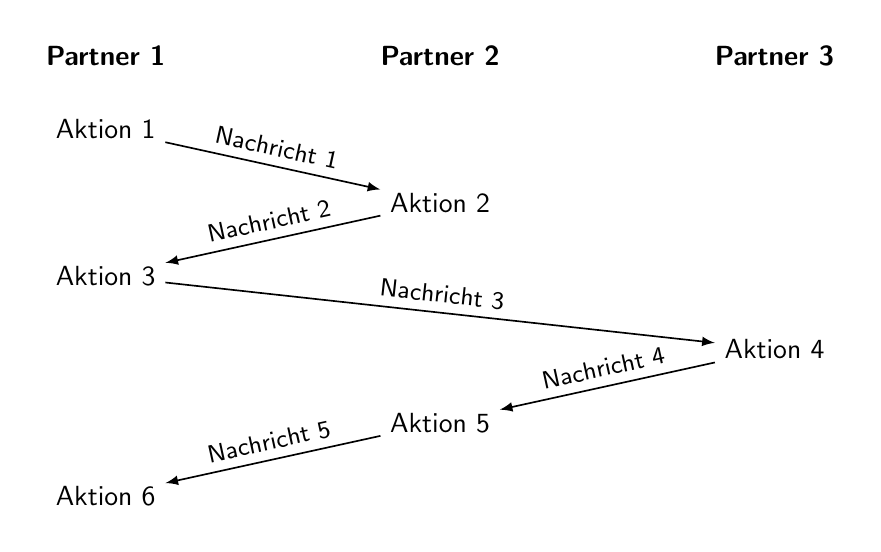
\begin{tikzpicture}[
every node/.append style={font={\sffamily}},
caption/.append style={font={\sffamily\bfseries}},
comm/.style={-latex,semithick},
msg/.style={midway,sloped,above,font={\sffamily\small}},
]
\matrix[row sep=3ex,column sep=25mm] {
\node[caption] {Partner 1};  & \node[caption] {Partner 2}; & \node[caption] {Partner 3}; \\
\node (A1) {Aktion 1}; & & \\
& \node (A2) {Aktion 2}; & \\
\node (A3) {Aktion 3}; & & \\
& & \node (A4) {Aktion 4};\\
& \node (A5) {Aktion 5}; & \\
\node (A6) {Aktion 6}; & & \\
};

\draw[comm] (A1)--(A2) node[msg] {Nachricht 1};
\draw[comm] (A2)--(A3) node[msg] {Nachricht 2};
\draw[comm] (A3)--(A4) node[msg] {Nachricht 3};
\draw[comm] (A4)--(A5) node[msg] {Nachricht 4};
\draw[comm] (A5)--(A6) node[msg] {Nachricht 5};

\end{tikzpicture}
	\caption{Netzwerkkommunikationsgraph mit TikZ}
  \label{fig:net-comm}
\end{figure}
Natürlich darf auch eine Übersicht über die KIT-Corporate-Identity-Farben
nicht fehlen (s. \cref{fig:kit-colors}).
\begin{figure}[tbp]\centering
  \tikzsetnextfilename{kit-colors}
	\begin{tikzpicture}[
box/.append style={rectangle,inner sep=0pt,outer sep=0pt,minimum size=1.5em,draw=none,fill=#1},
label/.style={font={\ttfamily\footnotesize},anchor=east},
caption/.style={font={\ttfamily\footnotesize},rotate=90,anchor=west}
]
\matrix[row sep=.2em,column sep=.2em] {
  &
\node[caption] {\textbackslash{}KITgreen...};      &
\node[caption] {\textbackslash{}KITblue...};       &
\node[caption] {\textbackslash{}KITblack...};      &
\node[caption] {\textbackslash{}KITpalegreen...};  &
\node[caption] {\textbackslash{}KITyellow...};     &
\node[caption] {\textbackslash{}KITorange...};     &
\node[caption] {\textbackslash{}KITbrown...};      &
\node[caption] {\textbackslash{}KITred...};        &
\node[caption] {\textbackslash{}KITlilac...};      &
\node[caption] {\textbackslash{}KITcyanblue...};   \\
\node[label] {};               &
\node[box=KITgreen      ] {};  &
\node[box=KITblue       ] {};  &
\node[box=KITblack      ] {};  &
\node[box=KITpalegreen  ] {};  &
\node[box=KITyellow     ] {};  &
\node[box=KITorange     ] {};  &
\node[box=KITbrown      ] {};  &
\node[box=KITred        ] {};  &
\node[box=KITlilac      ] {};  &
\node[box=KITcyanblue   ] {};  \\
\node[label] {...70};      &
\node[box=KITgreen70    ] {};  &
\node[box=KITblue70     ] {};  &
\node[box=KITblack70    ] {};  &
\node[box=KITpalegreen70] {};  &
\node[box=KITyellow70   ] {};  &
\node[box=KITorange70   ] {};  &
\node[box=KITbrown70    ] {};  &
\node[box=KITred70      ] {};  &
\node[box=KITlilac70    ] {};  &
\node[box=KITcyanblue70 ] {};  \\
\node[label] {...50};      &
\node[box=KITgreen50    ] {};  &
\node[box=KITblue50     ] {};  &
\node[box=KITblack50    ] {};  &
\node[box=KITpalegreen50] {};  &
\node[box=KITyellow50   ] {};  &
\node[box=KITorange50   ] {};  &
\node[box=KITbrown50    ] {};  &
\node[box=KITred50      ] {};  &
\node[box=KITlilac50    ] {};  &
\node[box=KITcyanblue50 ] {};  \\
\node[label] {...30};      &
\node[box=KITgreen30    ] {};  &
\node[box=KITblue30     ] {};  &
\node[box=KITblack30    ] {};  &
\node[box=KITpalegreen30] {};  &
\node[box=KITyellow30   ] {};  &
\node[box=KITorange30   ] {};  &
\node[box=KITbrown30    ] {};  &
\node[box=KITred30      ] {};  &
\node[box=KITlilac30    ] {};  &
\node[box=KITcyanblue30 ] {};  \\
\node[label] {...15};      &
\node[box=KITgreen15    ] {};  &
\node[box=KITblue15     ] {};  &
\node[box=KITblack15    ] {};  &
\node[box=KITpalegreen15] {};  &
\node[box=KITyellow15   ] {};  &
\node[box=KITorange15   ] {};  &
\node[box=KITbrown15    ] {};  &
\node[box=KITred15      ] {};  &
\node[box=KITlilac15    ] {};  &
\node[box=KITcyanblue15 ] {};  \\
};

\end{tikzpicture}
	\caption{KIT-Corporate-Identity-Farben}
  \label{fig:kit-colors}
\end{figure}

\section{Theoreme und Listings}

Für eine mathematische Ausarbeitung gibt es LaTeX-\glspl{umgebung}, um
\index{Satz|see{Theorem}}\index{Theorem}Sätze (Theoreme), \index{Lemma|see{Theorem}}Lemma,
\index{Beispiel|see{Theorem}}Beispiele etc. im üblichen Stil von
Mathematik-Büchern zu setzen und zu referenzieren. Vordefiniert sind die
\glspl{umgebung}
\begin{itemize}
  \item \texttt{theorem} für Sätze
  \item \texttt{definition} für Definitionen
  \item \texttt{lemma} für Lemma
  \item \texttt{corollary} für Korollare
  \item \texttt{proposition} für Propositionen
\end{itemize}
Die übliche Verwendung ist
\begin{latex}[caption={Beispiel für Theorem-Umgebungen},label={lst:ntheorem}]
\begin{theorem}[Optionaler Name]\label{thm:my-thoerem}
...
\end{theorem}
\end{latex}
Weitere Informationen findet man in der Dokumentation zum \texttt{ntheorem}-Paket
\parencite{May2011}. Das Ganze sieht dann beispielsweise wie folgt aus.

\begin{theorem}[Theorem von Arthur Dent]\label{thm:arthur-dent} Die Antwort auf
die Frage nach dem Leben, dem Universum und den ganzen Rest ist 42.
\end{theorem}

\begin{proposition}[Zweifelhafte Folgerung] LaTeX ist schön. Beweis folgt
unmittelbar aus \cref{thm:arthur-dent}.
\end{proposition}

Zum Einbinden und formatieren von \index{Code|see{Listing}}Code-Beispielen --
sog. \index{Listing}Listings -- wird das Paket \texttt{listings}
\parencite{Hoffmann2014} unterstützt. Das Hervorheben von
\index{Schlusselwort@Schlüsselwort}Schlüsselwörtern wird von LaTeX automatisch
erledigt, wenn die korrekte Sprache des Listings angegeben ist. Vordefininiert
sind die Umgebungen \texttt{java} für \gls{java} und \texttt{latex} für \gls{latex}.
Ein Beispiel
\begin{latex}[%
  caption={Listing-Beispiel},%
  label={lst:listing}]
\begin{java}[caption={A Java Hello-World example},label={lst:hello-world}]
public class HelloWorld {
  public static void main( String[] args ) {
    System.out.println( "HelloWorld" );
  }
}
\end{java}
\end{latex}
Das Ergebnis ist
\begin{java}[caption={A Java Hello-World example},label={lst:hello-world}]
public class HelloWorld {
  public static void main( String[] args ) {
    System.out.println( "HelloWorld" );
  }
}
\end{java}
Man beachte, dass anders als bei anderen Umgebungen die Bezeichnung
(\texttt{caption}) und die Referenzmarke (\texttt{label}) nicht als gesonderte
Befehle sondern als optionale Argumente übergeben werden. Dies liegt daran,
dass ein Listing in der Regel keine Fließumgebung ist, sondern an der Stelle
im Text erscheint, an der sie im Code auch steht. Ferner folgt ein Listing den
ganz normalen Seitenumbruchsregeln. Das heißt, überlanger Code wird einfach
umgebrochen. Um ein Listing zu einem Fließobjekt zu machen, muss das optionale
Argument \texttt{float=<tbp>} angegeben werden. Die
\index{Platzierung}Plazierungsangabe \texttt{h} für \enquote{hier} ist nicht
erlaubt. Denn dies ist das Standardverhalten ohne \texttt{float}.


\section{Literaturangaben}

Die Erstellung eines Literaturverzeichnisses geschieht mithilfe von \gls{biblatex}.
Hier soll an dieser Stelle nicht viel Erklärung dazugegeben werden, denn die
offizielle Dokumentation ist eine der besten Dokumentation, die ich überhaupt
kenne \parencite{Lehman2013}. Insbesondere seien die Abschnitte \enquote{3.7
Citation Commands} und das gesamte Kapitel \enquote{2 Database Guide} ans Herz
gelegt. Ersteres erklärt, wie im Text korrekt auf eine \index{Zitat}Zitatstelle verwiesen
wird, letzteres erklärt wie die BIB-Datei auszusehen hat.

Wer nicht die Originaldokumentation liest sondern nach irgendwelche (stets total
falschen) Lösungen im Internet sucht, weil er zu faul ist einfach nur mal lesen,
der hat mit Fug und Recht jede nur denkbare schlechte Note auf seine Arbeit
verdient.

\section{Stichwortverzeichnis (Index) und Glossar}

Die Vorlage unterstützt auch ein Stichwortverzeichnis und ein Glossar. Ein
Stichwortverzeichnis (oder Index) ist einfach nur eine alphabetisch sortierte
Liste von Begriffen mit einer Auflistung der \index{Fundstelle}Fundstellen
im Dokument. Ein Glossar ist eine alphabetisch sortierte Liste von Begriffen mit
\index{Erklarung@Erklärung}Erklärung.

Der Index wird erzeugt, indem im Quellcode der Befehl \verb#\index{Begriff}#
eingefügt wird. Wichtig, der Begriff selbst wird dadurch nicht gedruckt, sondern
muss noch einmal wiederholt werden, um auch gedruckt zu werden. Dieses Verhalten
ist beabsichtigt, sodass im Index immer nur die Grundform des Wortes verwendet
wird, aber im Text natürlich die richtige Deklination. Also:
\begin{latex}[caption={Beispiel für Index},label={lst:index}]
Die meisten Funktionen dieser \index{Vorlage}Vorlage, werden durch
\index{Paket}Standardpakete bereitgestellt.
\end{latex}
Obiges Beispiel erzeugt einen Indexeintrag für \enquote{Vorlage} der auf
\enquote{Vorlage} verweist und einen Eintrag \enquote{Paket} der auf 
\enquote{Standardpaket} verweist.

Um ein Glossar zu erzeugen, müssen die Glossarbegriffe zunächst definiert werden.
Dies geschieht in der Datei \texttt{./content/00-glossary-definitions.tex}.
Es gibt zwei Haupttypen von Glossarbegriffen: Abkürzungen (Akronyme) und allg.
Einträge (z.\,B. Fachtermini).

Abkürzungen werden mit
\begin{latex}[caption={Definition von Abkürzungen},label={lst:acro}]
\newacronym[%
  shortplural={AUen},%
  longplural={Abgasuntersuchungen}%
] {au}{AU}{Abgasuntersuchung}
\end{latex}
Die drei Hauptargumente sind in dieser Reihenfolge Marke, Abkürzung und
Ausschreibung. Optionale Argumente sind die kurze und lange Pluralform.

Allgemeine Glossarbegriffe werden mit
\begin{latex}[caption={Definition von allg. Glossareinträgen},label={lst:gls}]
\longnewglossaryentry{pkg}{%
  name={Paket},%
  plural={Pakete}}%
{%
  Hier folgt eine lange Definition, die auch mehr als einen
	Absatz beinhalten darf.
}
\end{latex}
erzeugt.

Im Text werden die Einträge durch den Befehl \verb#\gls{Marke}# verwendet.
Der wesentliche Unterschied zwischen einer Abkürzung und einem allg.
Glossareintrag ist, dass bei Abkürzungen bei erstmaliger Verwendung die
Abkürzung gedruckt und die Langform in Klammer dahinter gesetzt wird.
Bei allg. Glossareinträgen wird einfach nur der Name gesetzt. Statt
\verb#\gls{Marke}# gibt es noch viele weitere Befehle, um im Kontext des
umgebenen Textes die korrekte Pluralform, Großschreibung am Satzanfang, etc.
zu gewährleisten. Hierfür konsultiere man das Handbuch zum Paket \texttt{glossaries}
(Pluralform, sic!) \parencite{talbot2014}.

\section{Mathematik}

Grundsätzlich gilt, was in \parencites{ams1999a}{ams1999b} steht. In der Datei
\texttt{./preamble/05-math.tex} sind eine Menge Kurzkommandos definiert, um eine
einheitliche Typografie von \index{Skalar}Skalaren, \index{Vektor}Vektoren,
\index{Matrix}Matrizen, \index{Zufallsvariable}Zufallsvariablen etc.
zur vereinfachen. In diese Dateien einfach mal reinschauen, welche Kurzkommandos
es gibt.

Auf zwei besondere Kommandos wird näher eingegangen, weil dies häufig falsch
gemacht wird.
\begin{itemize}
  \item Für die Matrixtransponierte gibt es das Kommando \verb#\Tr#, also
	\verb#$\mA^{\Tr}$# liefert $\mA^{\Tr}$
	
	\item Bei \index{Integral}Integralen muss das \enquote{Differential-d} gemäß
	ISO in aufrechter Schrift als Operator gesetzt sein mit einem kleinen Abstand
	zum Integranden. Hierfür gibt es das spezielle Kommando \verb#\diff#. Also
	\begin{equation}
	 \int^1_0 x^2 d x = \frac{1}{3} \qquad \text{(falsche Typografie!)}
	\end{equation}
	ist falsch, während \verb#\int^1_0 x^2 \diff x = \frac{1}{3}# das Richtige
	liefert
	\begin{equation}
	 \int^1_0 x^2 \diff x = \frac{1}{3} \qquad \text{(richtige Typografie!)}
	\end{equation}
\end{itemize}

\section{Sonstiges (URLs, Anführungszeichen, Sprache und Randnotizen)}

Hier nur eine lockere Sammlung von kleineren Hinweisen, für die ein eigener
Abschnitt zuviel gewesen wäre.

\subsection{URLs}

\index{Internetadresse|see{URL}}Internetadressen werden in das Kommando \verb#\url{...}# eingefasst

\subsection{Anführungszeichen}

Um irgendwas in Anführungszeichen einzufassen, wird das Kommando 
\verb#\enquote{...}# verwendet. Dies hat den Vorteil, dass man sich nicht um die
korrekte typografische Variation der Anführungszeichen in Abhängigkeit der
\index{Sprache}Sprache kümmern muss und auch verschachtelte Anführungszeichen korrekt behandelt
werden. Also aus
\begin{latex}[caption={Behandlung von Anführungszeichen},label={lst:quotes},escapechar=\#]
 \enquote{Beim Erreichen der K#ü#ste sprach Hamlet: \enquote{Es ist etwas faul im Staate D#ä#nemark}}.
\end{latex}
wird \enquote{Beim Erreichen der Küste sprach Hamlet: \enquote{Es ist etwas faul
im Staate Dänemark}} mit korrekt verschachtelten einfachen Anführungszeichen.

\subsection{Sprachumschaltung (Deutsch, Englisch, etc.)}

Um für einen Teil des Textes die \index{Sprache}Sprache zu wechseln, damit die
\index{Silbentrennung}Silbentrennung und die Auswahl der Anführungszeichen
korrekt funktioniert, gibt es zwei Kommandos. Für einen kürzeren Text gibt es
\verb#\foreignlanguage[Sprache]{...}#. Dann wird für den Text in den
geschweiften Klammern die angegebene Sprache verwendet. Um die Sprache bis zum
nächsten Aufruf des gleichen Kommandos dauerhaft umstellen, gibt es
\verb#\selectlanguage{Sprache}#. Gegenwärtig unterstütze Sprachen sind
\texttt{ngerman} für Deutsch nach neuer
\index{Rechtschreibung!neue deutsche}Rechtschreibung und \texttt{american} für
Englisch nach amerikanischer \index{Rechtschreibung!amerikanisch}Rechtschreibung.

\subsection{Randnotizen}

Randnotizen werden mit dem Kommando \verb#\marginnote{...}# gesetzt\marginnote{Ich bin eine überflüssige Randnotiz}.
Diese eignet sich zum Beispiel um im Text Stellen zu kennzeichnen, an denen
man noch arbeiten sollte.
